\begin{figure}[b]
    \centering
    \begin{subfigure}{0.4\linewidth}
        \centering
        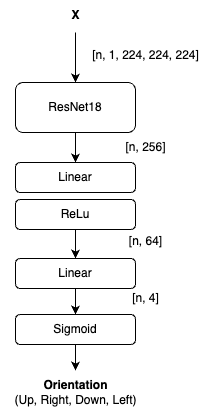
\includegraphics[width=\linewidth]{images/OrientationModel.png}
        \caption{Orientation Model}
        \label{fig:orientation_model}
    \end{subfigure}
    \begin{subfigure}{0.4\linewidth}
        \centering
        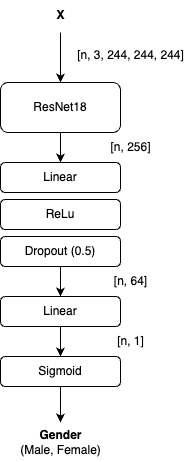
\includegraphics[width=\linewidth]{images/GenderModel.png}
        \caption{Gender Model}
        \label{fig:gender_model}
    \end{subfigure}
    \begin{subfigure}{0.4\linewidth}
        \centering
        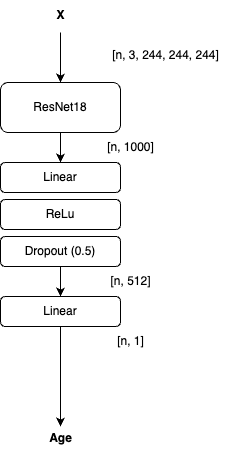
\includegraphics[width=\linewidth]{images/AgeModel.png}
        \caption{Age Model}
        \label{fig:age_model}
    \end{subfigure}
    % \begin{subfigure}{0.5\linewidth}
    %     \centering
    %     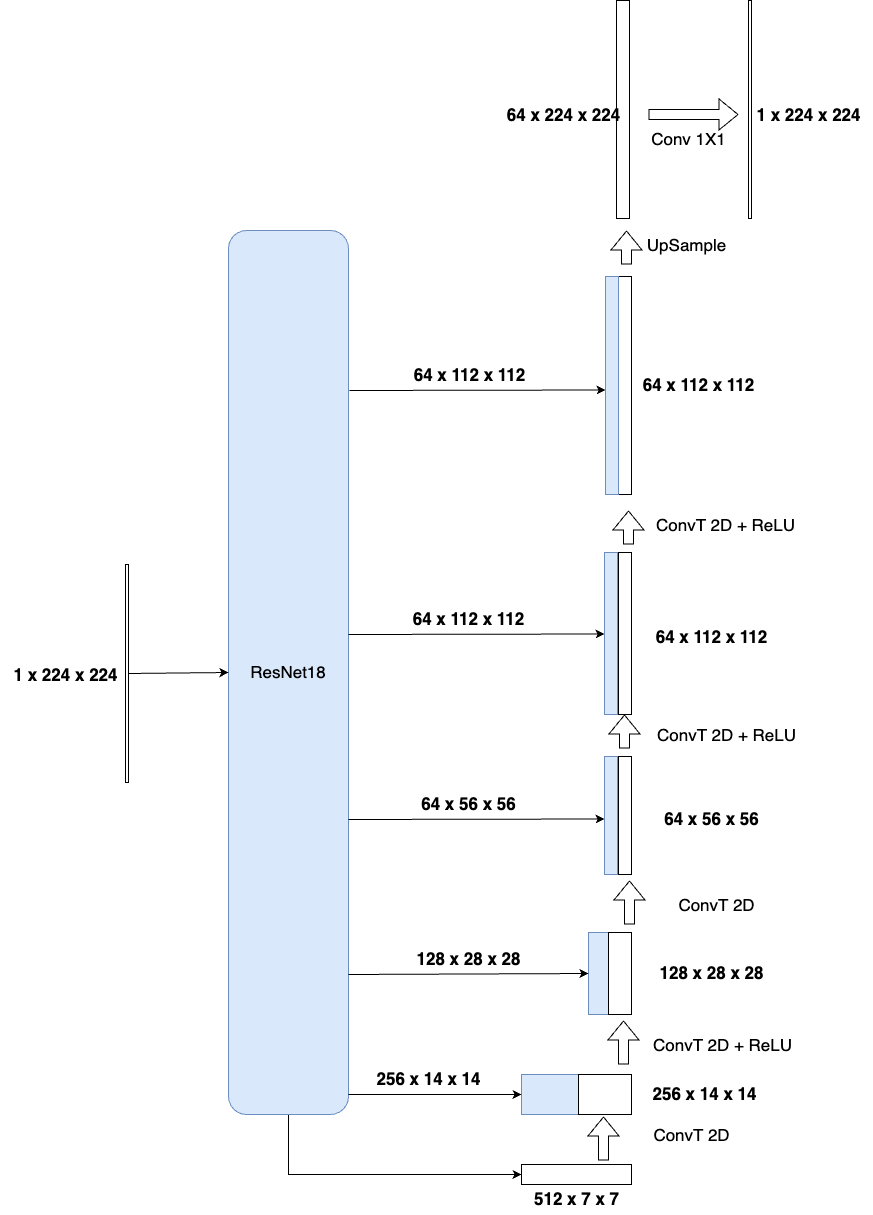
\includegraphics[width=\linewidth]{images/Unet-segmentation.png}
    %     \caption{UNet for lung segmentation}
    %     \label{fig:unet_lung}
    % \end{subfigure}
    
\end{figure}

\begin{figure}[htbp]
    \centering
    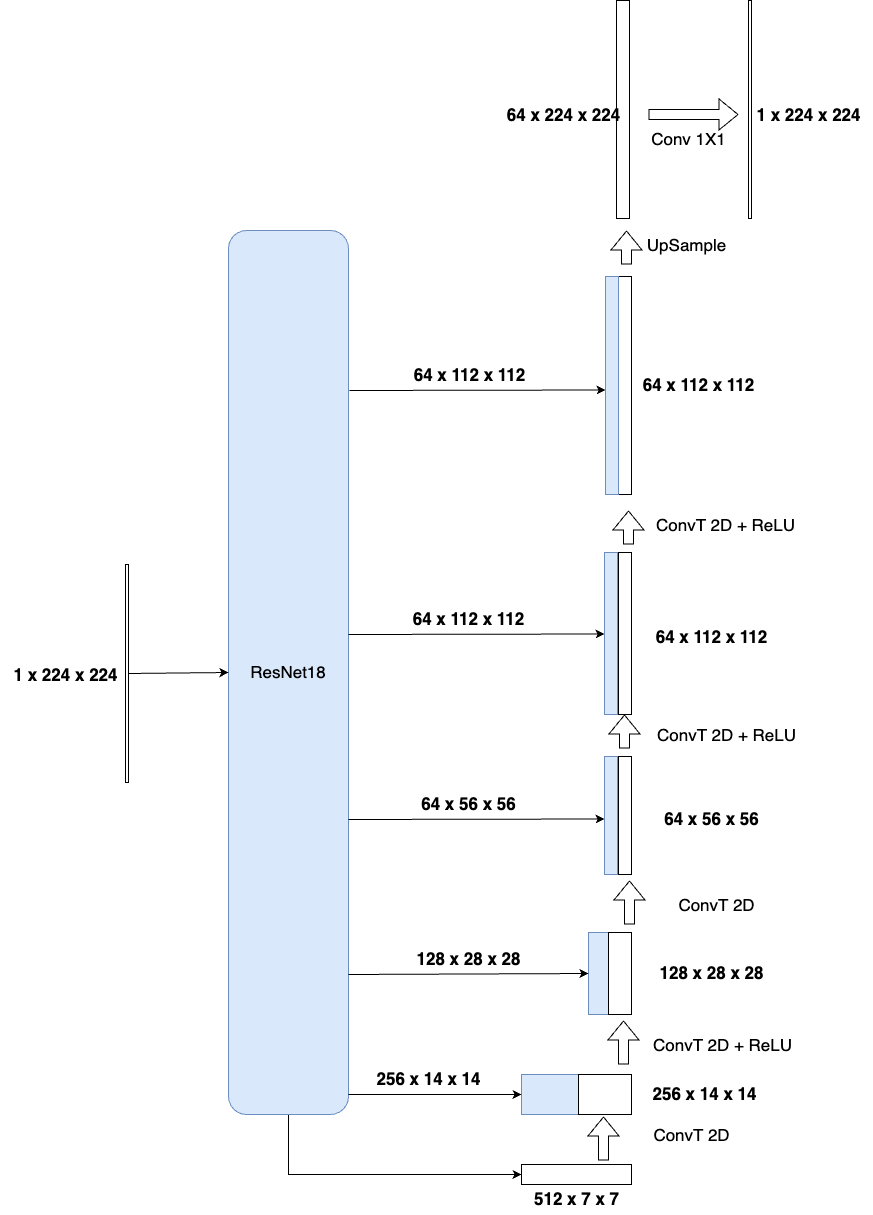
\includegraphics[width=\linewidth]{images/Unet-segmentation.png}
    \caption{UNet for lung segmentation}
    \label{fig:unet_lung}
\end{figure}